% =====================================================================
% ONR_white_paper.tex -- AICHAINS white paper, ONR BAA N0001425SB001,
%                    Mathematical Data Science (Code 311)
%
% Status: full prose draft, Oct 19, 2026 (LLM-artifact pass applied; see
% root LLM_ARTIFACT_REMOVAL.md and PROSE_STYLE_GUIDE.md). Target format:
% 8.5x11, 1-inch margins, single spaced, Times New Roman 12 pt; body
% ~2,400 words across 5 pages excluding cover. Placeholders marked
% [verify]. Figure: two-panel float --- (a) NDA-safe synthetic tree
% encoding; (b) agent-interface screenshot, NDA PLACEHOLDER the PI
% replaces before submission (fallback: figs/panel_b_tikz_backup.tex).
%
% BAA-mandated layout: cover page (page 0, unnumbered, not counted toward
% the limit), then body sections in order: 1. Technical Concept;
% 2. Future Naval Relevance; 3. Rough Cost Estimate. Operational Concept
% omitted (not applicable).
% =====================================================================
\documentclass[12pt]{article}
% Strict font compliance: BAA requires Times New Roman 12 pt -- use the actual
% system Times New Roman via XeLaTeX/fontspec (compile with: xelatex ONR_white_paper).
\usepackage[letterpaper,margin=1in]{geometry}
\usepackage{iftex}
\usepackage{url}
\urlstyle{same} % strict BAA font compliance: URLs in Times New Roman, not monospace
\ifXeTeX
  \usepackage{fontspec}
  \setmainfont{Times New Roman}  % real Times New Roman (BAA requirement)
\else
  % pdflatex fallback: metric-compatible Times clone; FINAL submission should be
  % compiled with xelatex so the embedded font is genuine Times New Roman.
  \usepackage{newtxtext,newtxmath}
\fi
\usepackage{graphicx}
\usepackage{tikz}
\usetikzlibrary{arrows.meta,positioning}
\usepackage[font=small]{caption}
\usepackage{cleveref}
\usepackage{titlesec}

% Plain, compact section headings (12 pt bold, word-processor style)
\titleformat{\section}[block]{\normalsize\bfseries}{}{0em}{}
\titlespacing*{\section}{0pt}{6pt plus 1pt}{4pt}

\emergencystretch=1em
\raggedbottom

% Engine-portable delta-t label for the figure (XeLaTeX renders the real
% Times New Roman glyph; pdfLaTeX falls back to math mode).
\ifXeTeX
  \newcommand{\deltat}{\textit{Δt}}
\else
  \newcommand{\deltat}{$\Delta t$}
\fi

\begin{document}

\thispagestyle{empty} \begin{center} \textbf{WHITE PAPER SUBMITTED IN RESPONSE TO}\\[4pt]
\textbf{ONR BAA N0001425SB001 (as amended by Amendment 0008, Sep 2026)}\\[4pt]
Program: Mathematical Data Science (Code 311) --- Dr.~Predrag Neskovic \end{center}

\vspace{0.6in}

\noindent\textbf{Title:} AICHAINS: AI Causal Hypothesis Analysis and Inference System---Certified Causal Root-Cause Analysis for Complex Systems with Guarantees

\vspace{0.25in}

\noindent\textbf{PI:} Bruno Ribeiro, Associate Professor, Computer Science, Purdue University\newline {ribeirob@purdue.edu} \textbar{} \url{https://www.cs.purdue.edu/homes/ribeirob/} \newline \textbf{Co-PI:} Sanjay Rao, Professor, Computer Science, Purdue University\newline {[}email, exact title --- verify{]} \newline Institutional contact: Purdue SPS {[}name/phone/email --- request{]}.

\vspace{0.25in}

\noindent Rough cost estimate: \$0.68M total over 3 years (about \$155K/year direct excluding student fee remissions and F\&A-excluded items, plus indirect at Purdue F\&A 57\% of MTDC; see Section 3).

\vspace{0.25in}

\noindent Topic areas addressed (per the Mathematical Data Science program page): \begin{itemize} \item Dynamical properties of networks and determination of causal effects \item Computational algorithms that scale to large networks with performance guarantees \end{itemize}

\vspace{0.25in}

\noindent Date: {[}submission date{]} \textbar{} Purdue UEI/CAGE: {[}request from SPS{]}

\newpage \setcounter{page}{1}




\section*{1. Technical Concept}

\textbf{The problem.} When a complex system degrades---a manufacturing line, a logistics network, a ship's propulsion plant, a communication network---the operational question is which node, change, or propagation chain caused the incident, and what it will affect next. Answering it requires correlating sensor telemetry, logs, tickets, and change records over time and across organizational boundaries; performed manually, this correlation is slow. In a recent diagnosis at Seagate's semiconductor manufacturing plant, an engineering team spent weeks on a single recurring defect, rerouting production while defects continued, without reaching closure.

Our industry experience with RCA (Ford, Seagate, Amazon) has shown us that RCA is well suited to agentic automation because it is an iterative, hypothesis-driven process: the analyst queries a data source, forms a suspicion, follows it into another source, and refines the hypothesis. The standard approach for such agents is retrieval-augmented generation (RAG): a vector index over \emph{text}---tickets, manuals, knowledge-base articles---queried at each RCA step. Current agentic and RAG architectures are mismatched to systems diagnosis in three respects. First, existing diagnostic tools are designed for human consumption: they collapse the space of candidate causes into a few point diagnoses, discarding the \emph{epistemic uncertainty}---uncertainty about what has not been observed---arising from uninstrumented steps, unlogged interventions, and dependencies absent from the recorded system map.

Second, multi-hop reasoning is difficult. Tickets omit technical context, change logs do not capture dependencies or all potential downstream consequences, and linking a symptom to a cause may traverse a chain of undocumented relationships. For example, if a part fails at inspection, the defect may have been introduced three process steps earlier by a tool, on specific machines, and only for lots that skipped an intermediate rework step. Third, current RAG operates on text and on sources convertible to text. It succeeds there because documents and knowledge bases are written for retrieval. A plant's diagnostic evidence---sensor tensors, dependency graphs, event chains, and unstructured logs---is not as easily retrievable with existing methods. What the agent must retrieve here is a structured \emph{candidate explanation for an issue}, together with related smaller issues---past or present---that have not yet surfaced, and the process changes that may have downstream consequences related to the issue. Existing agentic RAG solves only about 11\% of failure cases on the OpenRCA benchmark,\footnote{J.~Xu, Q.~Zhang, Z.~Zhong, S.~He, C.~Zhang, Q.~Lin, D.~Pei, P.~He, D.~Zhang, and Q.~Zhang, ``OpenRCA: Can Large Language Models Locate the Root Cause of Software Failures?,'' in \emph{Proc.\ Int.\ Conf.\ on Learning Representations (ICLR)}, 2025.} and a tree-search diagnostic agent that exceeds 90\% accuracy on an open benchmark loses about 26 points on production incidents.\footnote{A.~Naakka, Y.~Wang, and M.~V. M\"{a}ntyl\"{a}, ``LATS-RCA: Language Agent Tree Search for Root Cause Analysis in Microservices,'' in \emph{Proc.\ 52nd Euromicro Conf.\ on Software Engineering and Advanced Applications (SEAA)}, 2026; arXiv:2605.03505.} These three limitations have a common root: RCA is a \emph{causal inference} problem---genuine cause chains versus spurious correlation under partial observability---yet formal causal machinery and practical multimodal diagnosis pipelines have developed largely in isolation.

\begin{figure}[htbp]
\centering
\begin{minipage}[t]{0.42\textwidth} \centering
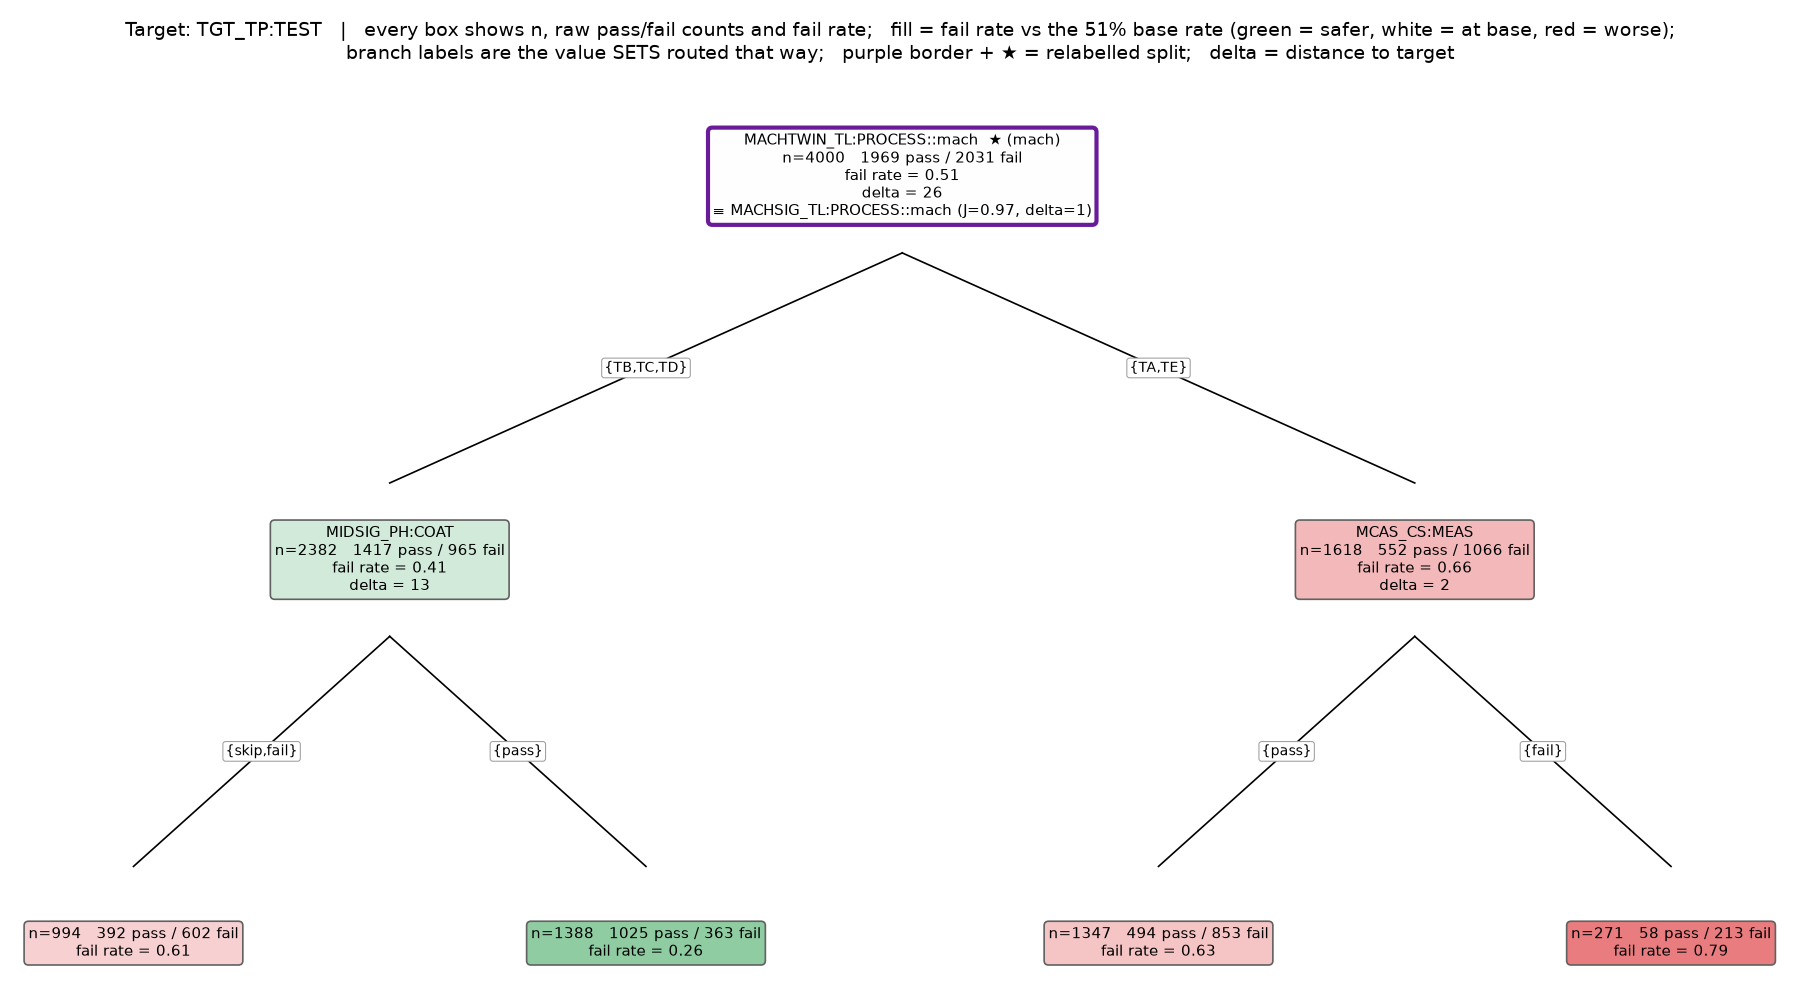
\includegraphics[width=\linewidth]{figs/aichains_tree_tree.png}\\[0pt]
{\small (a)}
\end{minipage}\hfill
\begin{minipage}[t]{0.34\textwidth} \centering
% PLACEHOLDER (NDA): AICHAINS agent-interface screenshot from the Birck poster
% (Sept 28, 2026; sensitivity-labeled, content NDA-gated). Shows the user
% asking which past steps explain failures at a target step and the agent's
% "Key Takeaways" answer including the abstention caution. The PI will
% replace this panel before submission. NDA-safe fallback: the synthetic
% TikZ incident-chain drawing saved in figs/panel_b_tikz_backup.tex.
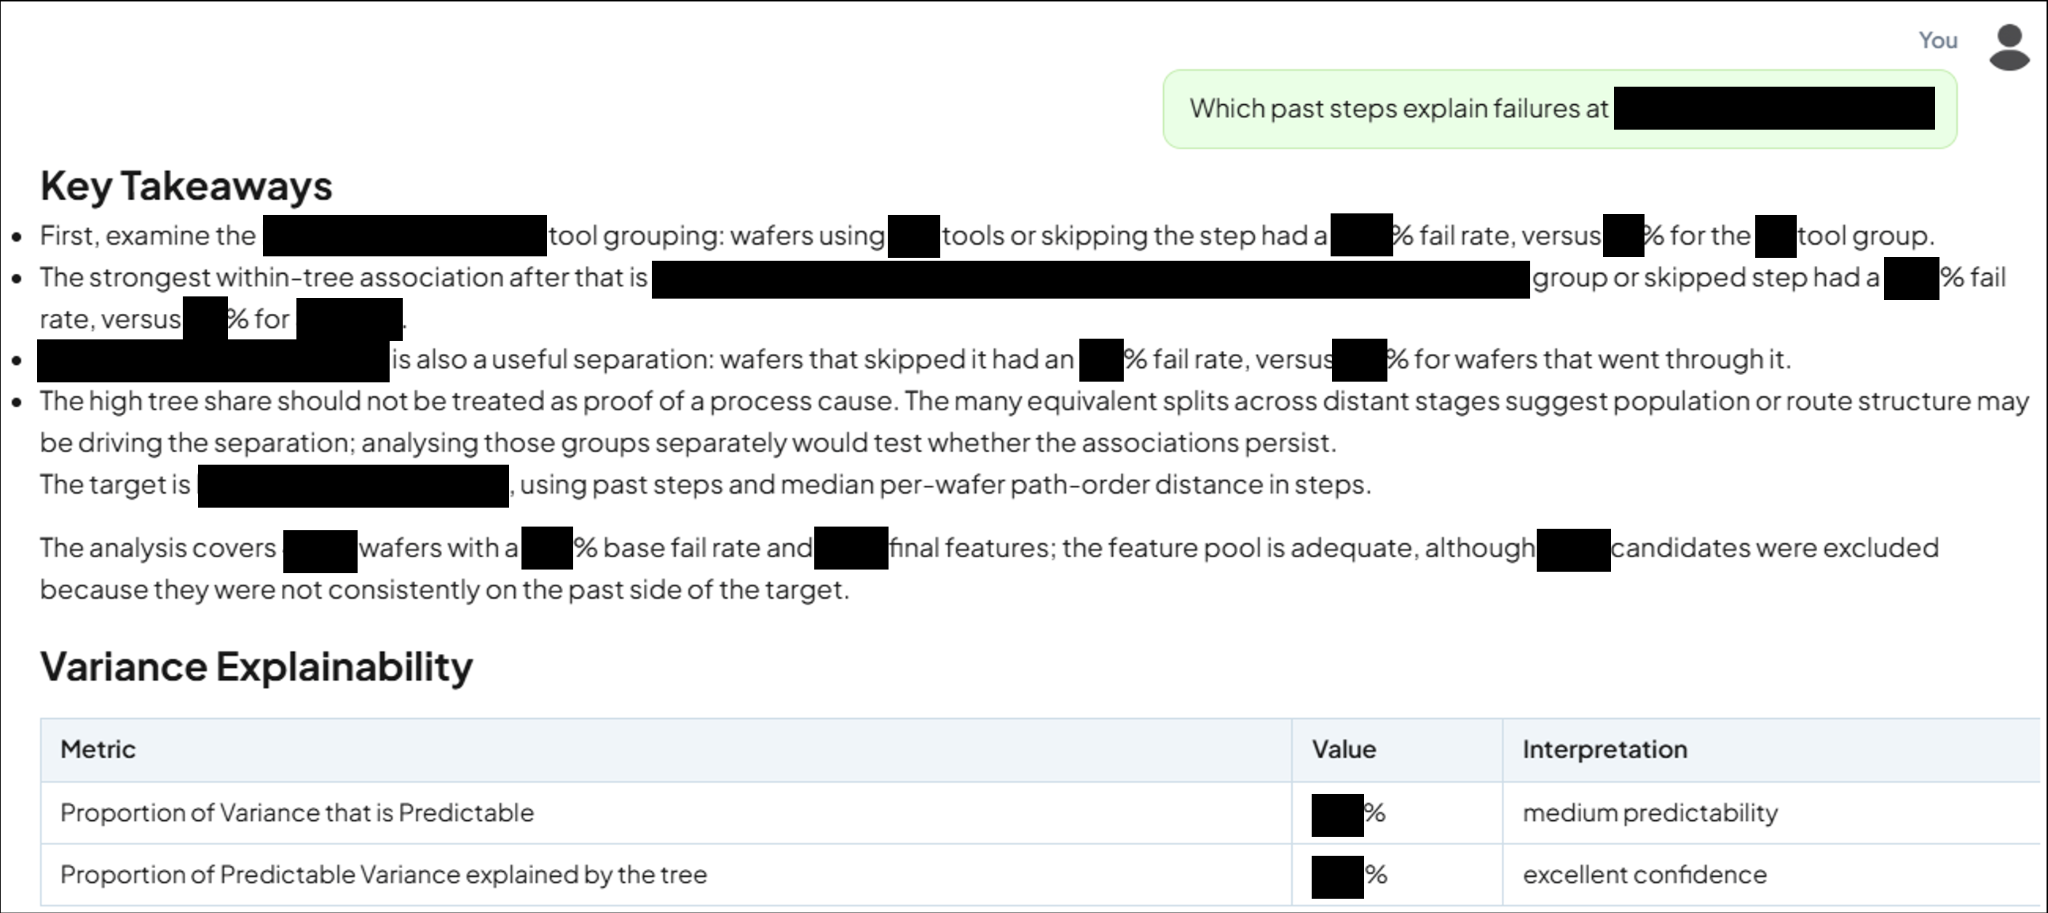
\includegraphics[width=\linewidth]{figs/aichains_agent_ui_NDA_PLACEHOLDER.png}\\[0pt]
{\small (b)}
\end{minipage}
\caption{The AICHAINS encoding and agent interface. (a) The interpretable encoding: a depth-limited pass/fail tree over wafer route history with positive set-based splits; each node reports the \emph{exhaustive set of equivalent splits} (two toolsets, Jaccard 0.97), preserving alternative explanations. (b) The agent interface: the user asks which past steps explain the failures at a target step; the agent answers with the strongest splits and their fail-rate contrast, and flags when a high tree share should not be read as proof of a process cause (abstention).}
\label{fig:aichains}
\end{figure}

\noindent
\textbf{The approach.} A complex system---a manufacturing line, a ship, a supply network---is a network of interacting components. Current diagnostic tools, including our deployed hypothesis-space system, establish \emph{associations}: they narrow a population of candidate explanations against the evidence, but a surviving hypothesis is a dependence pattern. The open problem is the passage from associations in hypothesis spaces to identifying causation: a candidate causal reason may already be present in the hypothesis space, and the task of the proposed research is to identify which mechanism the data support.

We claim certified RCA for such systems is achievable if we (1) represent the state of diagnosis as an explicit \emph{hypothesis space}---a structured, editable population of candidate causal incident chains that preserves, rather than prematurely collapses, epistemic uncertainty; (2) define \emph{operators} over these objects---intersection, temporal association, corpus-scale matching---with performance guarantees, so that the agent reasons with certified operators rather than with raw data; and (3) adjudicate the surviving hypotheses through \emph{causal verification}: causal discovery, from associational data, within the subpopulations (strata) that the hypothesis-space tree's splits define; interventional validation where feasible; and conformal abstention that bounds how often the system outputs a wrong or spurious cause.

Each step is a research contribution that, to our knowledge, no existing diagnostic system offers. (1) The encoding: diagnosis state is carried as a data-derived, editable population of candidate causal incident chains, and the same representation can absorb hand-authored procedures (playbooks, dependency maps, correlation rules) as further hypotheses. (2) The retrieval: operators match a hypothesis space to related hypothesis spaces. Each operator's specification states the structure of the hypothesis spaces it consumes and returns, what the output establishes (dependence structure, temporal precedence), and what it cannot (causation). Text RAG matches a query to documents and has no counterpart for hypothesis spaces. (3) The causal verification: the intersection of hypothesis spaces is an associational filter. The filter is designed not to eliminate the true cause: when the true cause is among the candidates in the space, that cause remains in the filter's output, alongside other associations that are not causal. This step determines which of the surviving chains are causal, through causal discovery within the subpopulations (strata) that the hypothesis tree's splits define, interventional validation where feasible, and conformal abstention. This is the step from association to causation that is key to delivering verifiable RCA answers.

We will develop AICHAINS (AI Causal Hypothesis Analysis and Inference System) to implement this approach. It addresses the program's two challenge areas: determination of causal effects in networks, by making the causal chain the primary object of inference; and algorithms that scale with performance guarantees, by requiring every operator to be typed and auditable and to carry distribution-free or structural guarantees.

\textbf{(1) Hypothesis spaces as populations of candidate causal chains.} A hypothesis space is the set of plausible failure modes consistent with observed data, encoded as time-indexed, text-annotated graphs satisfying three properties: (P1) capture relationships between hypotheses (refinements, subsumptions); (P2) stay compact---tree-like encodings over equivalent multi-feature splits avoid the combinatorial explosion of flat cross-products; (P3) preserve epistemic uncertainty---premature collapse of the space produces confident wrong diagnoses. Our preliminary deployed study illustrates (P3): an interpretable tree model over a manufacturing route-history dataset produced seven mutually incompatible explanations of one split, spanning hundreds of upstream operations. Reporting only the single best split would have yielded an incorrect root cause. AICHAINS advances this representation in a causal direction. Each hypothesis is an explicit \emph{incident chain}: a candidate causal mechanism with events, propagation edges, and timing. The space can thus contain a causal candidate without the data yet singling it out. We will develop techniques that find in the space the Markov equivalence classes supported by the data---those consistent with the observed conditional independence statements---and Thrust (3) then adjudicates the survivors. We will design two-part MDL encodings---a structure code over edges and timing, a residual code over events a chain leaves unexplained---so that model selection prunes the space while the reported equivalent splits mark what the data cannot distinguish. Chain structure is elicited jointly from data and domain experts through three-valued edge feedback (certainly, certainly not, maybe), extending our group's human-in-the-loop causal discovery line. The contribution here is the representation itself: an editable, uncertainty-preserving population of candidate causal chains, derived from data and expert elicitation, that no current diagnostic system maintains.

\textbf{(2) RAG over hypothesis spaces.} Text RAG matches a text query to documents, images, or videos. AICHAINS RAG matches the current hypothesis space to related hypothesis spaces: an elevated fail rate---whether or not it triggered a response---can be matched to similar episodes, past or still unfolding, and to the process changes that preceded it. Three operator families realize this matching, each with a formal specification. An operator is \emph{typed}: its specification declares the structure of the hypothesis spaces it consumes and returns, and carries an \emph{identifiability statement}---what the output licenses (dependence structure, temporal precedence) and what it cannot (causation, absent the verification of Thrust (3)). \emph{Intersection} retrieves the evidence for a hypothesis: it aligns symptom spaces (from live telemetry) against cause spaces (from change logs, tickets, association graphs) via graph transformers equivariant to the representation's symmetry group, fused with text encoders by cross-attention. Trees identical up to equivalent split orderings receive identical representations. We will characterize when the intersection is injective, so that every surviving hypothesis traces to exact supporting artifacts. \emph{Temporal association} retrieves a hypothesis's history: it composes static equivariant snapshot encodings through a graph-then-time framework into variable-size embeddings that localize when a hypothesis first appears, disappears, or generalizes. Temporal precedence is computed from the data. \emph{Corpus-scale matching} retrieves entire past hypothesis spaces: (set-of-matrices)/(set-of-matrices) matching over permutation-equivariant node-level embeddings, scored by subgraph-isomorphism networks and compressed with late-interaction scoring, pre-trained label-free from LLM reasoning traces of resolved incidents via Gumbel-Sinkhorn alignment. A retrieved space is treated as evidence to intersect, adapt, and verify. The operators are thus associational; they become causal through Thrust (3), which makes explicit where discovery assumptions (faithfulness, no unmeasured confounders) enter and what only an intervention can establish. Causal discovery is run within the strata that the hypothesis tree's splits define---the units sharing each split history---where conditioning on the splits reduces dimensionality and makes constraint-based and score-based discovery tractable on high-dimensional network data. The contribution here is retrieval itself: matching structured hypothesis spaces to each other, under operators with guarantees, has to our knowledge no existing counterpart.

\textbf{(3) Certified causal verification and abstention.} The agent operates directly on the hypothesis space, which serves as its state: the operators act as transitions over this state, and the agent's memory is a corpus of prior hypothesis spaces, retrieved by corpus-scale matching, that informs the analysis of each new incident. Every accepted diagnosis is accompanied by a machine-checkable chain: each surviving incident chain must (a) trace to provenance-verified artifacts, (b) pass structural invariants (typing, dataflow consistency, strictly-decreasing consistency residuals---discharged with an SMT solver), (c) pass temporal precedence against the incident onset, and (d) survive \emph{interventional validation} where feasible---seeded fault injection in test systems and natural experiments in operation. Reliability scores are mapped to decisions through conformal prediction with ordering-invariant score functions, yielding distribution-free coverage and a calibrated \emph{abstain-or-escalate} verdict: when the surviving space still contains incompatible chains with incompatible interventions, the system escalates to a human with the ambiguity made explicit rather than an unsupported verdict. Faithfulness probes (counterfactual ablation of claimed causal edges) guard against post-hoc rationalization. The contribution here is the causal layer: deciding which chains surviving the intersection are causal, with bounded error or an explicit abstention. \Cref{fig:aichains} shows the two artifacts of the proposed research: the interpretable encoding and the agent interface through which users query it.

\textbf{Feasibility.} The proposed research builds on validated prior work: the PI's group authored the underlying representation theory (Holographic, ICLR 2025; STAGE, ICML 2025; All-IN, ICLR 2026), the temporal equivariance framework underlying temporal association, a human-in-the-loop causal discovery program, and PRISM, a video streaming RCA system the PI's and Co-PI's groups built with a major video-streaming provider. A system implementing the tree-based hypothesis-space diagnosis loop---the associational stage of the proposed program---is deployed in Ford's INSIGHT tool under a previous grant, and a version for semiconductor manufacturing is in development with Seagate (data under NDA). Its architecture separates inference from computation by design. The LLM agent only selects and parameterizes deterministic analysis tools, accessed through typed tool interfaces with read-only enforcement; every number an engineer sees comes from the analysis code rather than from the model. The trees use positive set-based splits and report the \emph{exhaustive set of equivalent splits} at every node. Strict leakage gates drop any candidate event that occurs after the target for even one unit (which is a consequence rather than a root cause). Confidence is scored as an entropy capture ratio against a gradient-boosting ceiling with a Nadeau–Bengio corrected significance test. Finally, results are deterministic: a cache keyed on data, parameters, and code digests returns identical answers in 0.02 s versus about 25 s of fresh analysis at production scale. The system is air-gapped with a local LLM, so data never leaves the site. The system was built to four design requirements (provenance, adaptability, reliability, uncertainty quantification) and was evaluated against real engineering-team investigations and synthetic data with by-construction root causes. PRISM found multiple simultaneous issues, including tail incidents missed by strong baselines, on real production snapshots.\footnote{C.~Bothra, X.~Jiang, Y.~Zhang, Z.~Akhtar, S.~G.~Rao, and B.~Ribeiro, ``PRISM: Localizing performance anomalies for large scale video services,'' manuscript in preparation, 2026.}

\textbf{Technical risk areas and mitigations} (per the BAA). (i) \emph{Discovery under confounding:} constraint-based discovery on observational fab/network data may be unfaithful. Mitigation: discovery runs within the hypothesis tree's strata, under stated assumptions, is validated interventionally where feasible, and never overrides provenance and precedence checks; it ranks candidates rather than certifying them. (ii) \emph{Hypothesis explosion:} intersecting multimodal spaces may explode combinatorially. Mitigation: compactness-by-construction encodings with tunable resolution (coarser or finer) let the agent control search breadth under explicit query budgets. (iii) \emph{Elicitation noise:} expert/LLM edge feedback is fallible. Mitigation: three-valued feedback feeds a contradiction registry; edges carry confidence and provenance; the conformal layer absorbs residual uncertainty. (iv) \emph{Integration risk:} the proposed operators and the causal-verification layer are yet to be developed, and their integration with the deployed associational stage is unproven; the seeded fault-injection protocol and pre-registered success criteria make the claim falsifiable.

\section*{2. Future Naval Relevance}

Root-cause analysis under time pressure is a recurring naval problem. A frigate's propulsion plant, a shipyard's build schedule, a semiconductor fab's yield line, and a sustainment network are each graphs of interacting components whose failures must be explained from sparse, noisy, multimodal evidence, typically without ground truth for the most consequential failure modes. AICHAINS is designed for this setting; we develop it across four naval problem classes, with manufacturing as the bridge domain (deployed in Ford's INSIGHT tool; in development for semiconductor manufacturing with Seagate).

\textbf{Naval platform health and condition-based maintenance (primary use case).} A ship's propulsion plant is a dependency graph of sensors, actuators, and subsystems; a combat system, a chain of processing, power, and cooling dependencies. When a casualty occurs, the questions are which chain of events produced the anomaly, which subsystems it will affect, and what to inspect first. AICHAINS maintains and edits populations of candidate failure-propagation chains over the platform's dependency graph. Intersection aligns live telemetry against maintenance and configuration changes. Temporal association localizes when a propagating degradation began. The certified chain gives the watch team a defensible answer with a bounded error rate or, when evidence is insufficient, an explicit statement of the surviving ambiguity.

\textbf{Naval manufacturing, shipyard repair, and trusted microelectronics (bridge domain).} The PI's group operates a deployed, regression-tested RCA system of the proposed hypothesis-space loop in Ford's INSIGHT tool (from a previous grant), and a version for semiconductor manufacturing is in development with Seagate (data under NDA; described at problem-class level). These systems address the same problem class as naval manufacturing and repair. Shipyard workflows, depot overhaul, naval additive manufacturing, and trusted microelectronics production are process-dependency graphs: defects propagate across stages, tools, and lots, and yield is lost to failures invisible in the final product. Transfer to the naval setting is supported by attribute-domain-agnostic representations rather than by domain-specific engineering. These systems demonstrate the methods under industrial constraints: audit trails, deterministic reproducibility, air-gapped operation, and a design rule that the system never claims causation from association. This proposal adds the formal causal machinery that removes that constraint.

\textbf{Fleet sustainment and logistics networks.} A strike group's sustainment is a multi-echelon supply network; parts flow and maintenance scheduling form a transport network over the platform graphs. Delay, disruption, and root-cause prediction reduce to the same problem: localizing fault propagation on a process-dependency graph from noisy, label-scarce observations, with the same certified-trace and abstention guarantees.

\textbf{Resilient shipboard computing.} Operators under explicit budgets define a compute-allocation policy for power-constrained platforms: diagnosis runs on frozen models, adapting only at test time. The certified chain is a shared human-machine artifact: every step is an auditable tool call, and every escalation carries the unresolved hypothesis space rather than an unprovenanced verdict.

\textbf{Program alignment.} These use cases fall within the program's Complex Networks concentration area (basic research on the dynamical properties of networks and the determination of causal effects, and on algorithms that scale with performance guarantees). They also bear on multi-modal information integration and decision making under uncertainty, through causal determination from system and network dynamics and scalable inference with guarantees. The research is basic: whether a population of associational hypotheses can be certified as causal---identifiability, compactness, and the guarantee theory required for trustworthy agentic diagnosis---is a foundational question for any naval deployment of diagnostic AI.

\textbf{Dual-use breadth.} The INSIGHT deployment at Ford and the system in development for Seagate demonstrate direct transfer of the research to U.S. industry; the PI further engages U.S. manufacturers through a co-authored NIST report and a 2026 U.S. Department of Commerce webinar for Indiana manufacturers.

\section*{3. Rough Order of Magnitude (ROM) Cost Estimate}

Faculty effort: PI (0.46 summer person-months/year, 3.85\% effort), Co-PI Sanjay Rao (effort to be set --- [verify]; current figures exclude Co-PI salary), two PhD students (4.5 academic-year months plus 3 summer months in Years 1–2; academic year only in Year 3), no postdoc. Direct costs: salaries and fringe benefits, graduate fee remissions, HPC compute (Purdue Gautschi Center), cloud storage, travel (1–2 conferences and one ONR review meeting/year). Indirect costs at Purdue's negotiated rate of 57\% of MTDC (DHHS-approved 10/03/2022). Figures are current Purdue SPS estimates; a full R\&R budget follows in any invited application.

\begin{center} \footnotesize \begin{tabular}{lccc} \hline Year & Direct & Indirect (57\% MTDC) & Total \\
\hline
Y1 & \$168,560 & \$77,041 & \$245,601 \\
Y2 & \$173,566 & \$79,895 & \$253,461 \\
Y3 & \$122,869 & \$54,041 & \$176,910 \\
Total & \$464,995 & \$210,977 & \$675,972 \\
\hline \end{tabular} \end{center}

\end{document}
